% Copyright 2013 Nicolai Hähnle <nhaehnle@gmail.com>
%
% This work is licensed under the Creative Commons Attribution-ShareAlike 3.0
% Unported License, see http://creativecommons.org/licenses/by-sa/3.0/
%
% Among other things, this means that yes, you may take e.g. illustrations from
% the book and use them in your own work. However, (a) you must give proper
% attribution by naming me as its original author and (b) you must make your
% derivative work available under the same or similar license terms.
%
% See the Creative Commons website for the exact licensing terms.

\chapter{Dual lattices and Fourier analysis}
\label{chapter:dual-lattices}

Consider the problem of integer programming or, more generally, lattice programming:
given a closed convex set $K$ and a lattice $\Lambda$,
decide whether there exists a lattice point $x \in K \cap \Lambda$.
A natural approach to deciding this problem
is to slice $K$ along translates of a lattice hyperplane,
analogous to the nearest-plane approach to the closest vector problem.
Each of the slices intersecting $K$ leads to an integer programming problem
of lower dimension.
\begin{center}
  \begin{tikzpicture}
    \draw[thick,fill=black!10]
      (0,0) -- (2,-1.3) -- (5,-0.2) node[below right] {$K$} arc[start angle=-50, end angle=10, radius=2cm]
      -- (3,2) -- (1,1.8) -- cycle;

    \draw (6,1.5) node[right] {$y^Tx = \alpha \in \Z$};
    \draw[->] (-0.5,0.1) -- node[left,near end] {$y$} +(0.1,-0.5);
    \clip (-1,-2) rectangle (6,2.5);
    \foreach \t in {-3,-2,-1,0,1,2}
      \draw ($(-1,0) + \t*(0,1.2)$) -- +(7,1.4);
  \end{tikzpicture}
\end{center}
These translates of lattice hyperplanes are defined by equations $y^Tx = \alpha \in \Z$,
where $y \in \R^d$ satisfies $y^Tx \in \Z$ for all $x \in \Lambda$.
This is one justification for the definition of \emph{dual lattices},
which we study in this chapter.

The running time of this particular approach to integer programming
depends strongly on how many lattice hyperplanes intersect $K$.
Fourier analysis neatly relates a lattice and its dual,
which allows us to bound the number of lattice hyperplanes that must be investigated.


\section{The dual lattice}

\begin{definition}
  Let $\Lambda \subset \R^d$ be a full dimensional lattice.
  Its \emph{dual lattice} is given by
  \[
    \Lambda^\star := \{ y \in \R^d ~:~ \forall x \in \Lambda:\, y^Tx \in \Z \}
  \]
\end{definition}

\begin{lemma}
  \label{lemma:dual-basis}
  Let $B \in \R^{d \times d}$ be a basis of $\Lambda$.
  Then $\Lambda^\star = \Lambda(B^{-T})$.
  In particular, $\Lambda^\star$ is a lattice.
\end{lemma}
\begin{proof}
  Let $c_1, \ldots, c_d$ be the columns of $B^{-T}$.
  \[
    \begin{array}{|c|}
      \hline \quad c_1^T \quad  \\\hline
      \vdots \\\hline
      c_d^T \\\hline
    \end{array}
    \cdot
    \begin{array}{|c|c|c|}
      \hline  & &\\[0.5em]
      b_1 & \dots & b_d \\
      & & \\[0.5em]\hline
    \end{array}
    =
    \begin{array}{|lcr|}
      \hline 1 & & 0 \\
       & \ddots & \\
      0 & & 1 \\\hline
    \end{array}
  \]
  Let $y \in \Lambda^\star$.
  Since the $c_1, \ldots, c_d$ form a basis of $\R^d$,
  we can write
  \[
    y = \alpha_1 c_1 + \dots + \alpha_d c_d,\, \alpha_j \in \R
  \]
  It suffices to show that all $\alpha_j \in \Z$,
  which follows from
  \[
    \Z \ni y^T b_j = \alpha_1 c_1^T b_j + \dots + \alpha_d c_d^T b_j = \alpha_j.
  \]
  Now suppose $y \in \Lambda(B^{-T})$, that is,
  we can write
  \[
    y = \alpha_1 c_1 + \dots + \alpha_d c_d,\, \alpha_j \in \Z
  \]
  Let $x \in \Lambda$, that is,
  \[
    x = \beta_1 b_1 + \dots + \beta_d b_d,\, \beta_j \in \Z
  \]
  Then
  \[
    y^Tx = \alpha_1 \beta_1 + \dots + \alpha_d \beta_d \in \Z
  \]
  That is, $y^Tx \in \Z$ for all $x \in \Lambda$,
  hence $y \in \Lambda^\star$ by definition.
\end{proof}

\begin{corollary}
  \label{corollary:transformed-dual-lattice}
  Let $\Lambda \subset \R^d$ be a full-dimensional lattice.
  \begin{enumerate}
    \item $\det \Lambda^\star = \frac{1}{\det \Lambda}$.

    \item $(\Lambda^\star)^\star = \Lambda$.

    \item Let $M \in \R^{d\times d}$ be an invertible matrix.
      Then $(M \Lambda)^\star = M^{-T} \Lambda^\star$.

    \item $(\alpha \Lambda)^\star = \frac{1}{\alpha} \Lambda^\star$ for $\alpha > 0$.
  \end{enumerate}
\end{corollary}

Intuitively, a dense lattice has a sparse dual and vice versa.
Two aspects of this connection are formalized in the Corollary,
but it can also be seen in the lattice hyperplanes corresponding to dual lattice vectors.
For a given $y \in \Lambda^\star$,
the distance between adjacent lattice hyperplanes $y^Tx = \alpha$ and $y^Tx = \alpha + 1$
for $\alpha \in \Z$ is $1 / \|y\|_2$.
In a dense lattice, lattice hyperplane translates must lie close to each other,
which means that dual lattice vectors must be long.
We will develop more statements of this form throughout this chapter.



\section{Successive minima and covering radius}

Let us define some measures of the overall sparsity of a lattice.

\begin{definition}
  Let $\Lambda \subset \R^d$ be a full-dimensional lattice.
  The \emph{successive minima} $\lambda_1, \ldots, \lambda_d$ of $\Lambda$ are
  \[
    \lambda_j(\Lambda) := \min\{ r > 0 ~:~ \dim( \Lambda \cap B(0,r) ) \geq j \}
  \]
  where the dimension is the dimension of the linear span of the lattice points
  of norm at most $r$.

  The \emph{covering radius} of $\Lambda$ is the maximal distance from the lattice:
  \[
    \mu(\Lambda) := \max_{p \in \R^d} d(p, \Lambda)
  \]
  When the lattice is clear from the context,
  we write $\lambda_1, \ldots, \lambda_d$ and $\mu$.
  Furthermore, we write $\lambda_j^\star$ and $\mu^\star$ for the corresponding
  quantities of the dual lattice.
\end{definition}

The covering radius can be equivalently defined as the smallest radius $r$
such that the union of balls of radius $r$ around each lattice point
covers the entire space -- hence its name.

\begin{example}
  \label{example:rect-lattice-minima}
  The lattice $\Lambda := \Lambda \begin{pmatrix} 1 & 0 \\ 0 & 3 \end{pmatrix}$
  satisfies $\lambda_1 = 1$, $\lambda_2 = 3$, and $\mu = \sqrt{10}/2$.
  \begin{center}
    \begin{tikzpicture}
      \foreach \x in {-2,-1,...,2.1}
        \foreach \y in {-1,0,1}
          \fill ($\x*(0.5,0) + \y*(0,1.5)$) circle[radius=2pt];

      \draw (0,0) node[below] {$0$};

      \draw (0.25,0.75) circle[radius=0.76cm];
      \fill (0.25,0.75) circle[radius=2pt] node[right] {$p$};
    \end{tikzpicture}
  \end{center}
\end{example}

As the example shows,
$\lambda_1$ is the length of a shortest vector,
but $\lambda_2$ need not be the length of a ``second-shortest'' vector.
Instead, it is the length of a shortest vector among all vectors that are
linearly independent from a shortest vector.
In general,
we can choose linearly independent vectors $v_1, \ldots, v_d \in \Lambda$ with $\|v_j\|_2 = \lambda_j$.
Such a set of vectors is called a set of \emph{shortest independent vectors} of the lattice.
An exercise shows that such a set need \emph{not} be a basis of the lattice.

\begin{lemma}
  \label{lemma:mu-lambda-d}
  Let $\Lambda$ be a $d$-dimensional lattice.
  Then $\mu \geq \lambda_d / 2$.
\end{lemma}
\begin{proof}
  All lattice points in the interior of the ball of radius $\lambda_d$ around the origin
  lie in a hyperplane $H$.
  A point at distance $\lambda_d/2$ from $H$ has distance at least $\lambda_d/2$ to the lattice,
  see Figure~\ref{fig:mu-vs-lambda-d}.
\end{proof}
\begin{figure}
  \begin{center}
    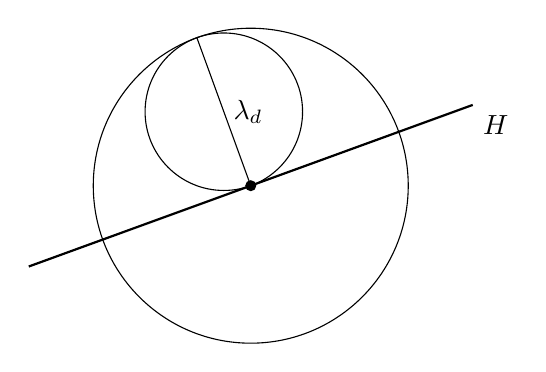
\begin{tikzpicture}
      \fill (0,0) circle[radius=2pt];
      \draw (0,0) circle[radius=2cm];
      \draw[thick] (20:-3) -- (20:3) node[below right] {$H$};

      \draw (0,0) -- node[right] {$\lambda_d$} (110:2);
      \draw (110:1) circle[radius=1cm];
    \end{tikzpicture}
  \end{center}
  \caption{The proof that $\mu \geq \lambda_d / 2$.}
  \label{fig:mu-vs-lambda-d}
\end{figure}

The lattice $\Z$ shows that the inequality of this Lemma is tight.
Let us now relate quantities of a lattice and its dual.
The following Lemma shows that a lattice and its dual cannot be too dense at the same time.

\begin{lemma}
  \label{lemma:transference-lower-bound}
  Let $\Lambda \subset \R^d$ be a full-dimensional lattice.
  Then $\lambda_1^\star \cdot \lambda_d \geq 1$,
  and hence $\lambda_1^\star \cdot \mu \geq 1/2$.
\end{lemma}
\begin{proof}
  Let $y \in \Lambda^\star$ be a shortest vector
  and let $v_1, \ldots, v_d \in \Lambda$ be shortest independent vectors.
  Since the $v_j$ form a basis of $\R^d$,
  we must have $y^T v_k \neq 0$ for at least one $k$.
  Using the Cauchy-Schwarz inequality and the fact that $y^T v_k \in \Z$,
  we can compute
  \[
    1 \leq |y^T v_k| \leq \|y\|_2 \|v_k\|_2 = \lambda_1^\star \lambda_k \leq \lambda_1^\star \lambda_d \qedhere
  \]
\end{proof}

\begin{example}
  Consider $\Lambda = \Lambda \begin{pmatrix} 1 & 0 \\ 0 & M \end{pmatrix}$ for $M > 1$.
  We have $\Lambda^\star = \Lambda \begin{pmatrix} 1 & 0 \\ 0 & M^{-1} \end{pmatrix}$
  and therefore
  \begin{align*}
    \lambda_1 &= 1 \\
    \lambda_d &= M \\
    \lambda_1^\star &= M^{-1} \\
    \lambda_d^\star &= 1
  \end{align*}
  That is, the inequality of Lemma~\ref{lemma:transference-lower-bound} is tight,
  both when applied to $\Lambda$ and when applied to $\Lambda^\star$.
\end{example}

We are interested in analogous statements showing
that a lattice and its dual cannot be too \emph{sparse} at the same time.
That is, we would like to have an \emph{upper bound} on a product of the form $\lambda_1^\star \cdot \lambda_d$.
Some bounds of this type are shown in the exercises of this chapter,
using Minkowski's theorem and LLL-reduced bases.
We will derive a much stronger bound in Section~\ref{sec:transference-bound-banaszczyk}.



\section{Lattice width and Flatness theorems}

We will now tie dual lattices and the quantities defined in the last section
together with the approach to integer programming based on lattice hyperplanes.

\begin{definition}
  Let $K \subset \R^d$ be a convex body.
  Let $\Lambda$ be a full-dimensional lattice and let $y \in \Lambda^\star$.
  The \emph{lattice width of $K$ with respect to $y$} is
  \[
    w_y(K, \Lambda) := \max_{x \in K} y^T x - \min_{x \in K} y^T x
  \]
  The \emph{lattice width of $K$} is
  \[
    w(K, \Lambda) := \min_{y \in \Lambda^\star \setminus \{0\} } w_y(K,\Lambda)
  \]
  We write $w_y(K)$ or $w(K)$ when the lattice is clear from the context.
\end{definition}

The lattice width with respect to $y \in \Lambda^\star$
describes the distance in terms of lattice hyperplanes between parallel planes
sandwiching the convex body.
This width is particularly easy to compute for a ball $B(z,r)$,
see Figure~\ref{fig:lattice-width-ball}:
\begin{align*}
  w_y(B(z,r)) &= \max_{x \in B(z,r)} y^Tx - \min_{x \in B(z,r)} y^Tx \\
   &= y^T (z + r \frac{y}{\|y\|_2}) - y^T (z - r \frac{y}{\|y\|_2}) \\
   &= 2r \frac{y^T y}{\|y\|_2} = 2r \|y\|_2
\end{align*}
\begin{figure}
  \begin{center}
    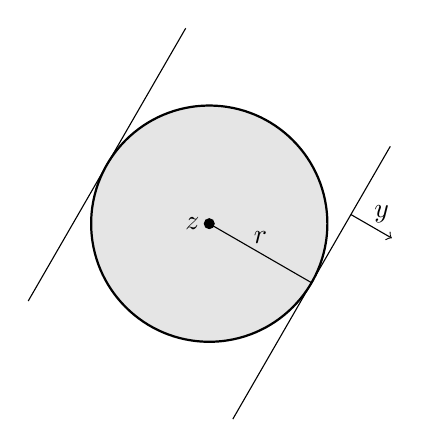
\begin{tikzpicture}
      \draw[thick,fill=black!10] (0,0) circle[radius=1.5cm];
      \fill (0,0) circle[radius=2pt] node[left] {$z$};
      \draw (-30:1.5) +(60:-2) -- +(60:2);
      \draw (-30:-1.5) +(60:-2) -- +(60:2);
      \draw[->] (-30:1.5) ++(60:1) -- node[above,near end] {$y$} +(-30:0.6);
      \draw (0,0) -- node[above] {$r$} (-30:1.5);
    \end{tikzpicture}
  \end{center}
  \caption{The lattice width of a ball with respect to $y \in \Lambda^\star$.}
  \label{fig:lattice-width-ball}
\end{figure}

\begin{lemma}
  The lattice width of a ball of radius $r$ is $2r\lambda_1^\star$.
\end{lemma}
\begin{proof}
  \[
    w(B(z,r)) = \min_{y \in \Lambda^\star \setminus \{0\} } w_y(B(z,r))
      = \min_{y \in \Lambda^\star \setminus \{0\} } 2r \|y\|_2 = 2r \lambda_1^\star
    \qedhere
  \]
\end{proof}

Since the lattice width is invariant under linear transformations (see the exercises),
this result easily extends to ellipsoids.
Intuitively, we can find the lattice width of an ellipsoid $E$
by finding a matrix $A$ such that $A \cdot E$ is a ball
and then computing a shortest vector in $A^{-T} \cdot \Lambda^\star$,
the dual lattice of $A \cdot \Lambda$.

\begin{theorem}[Flatness Theorem for Ellipsoids]
  \label{thm:flatness-ellipsoids}
  Let $d \in \N$.
  Suppose there is a constant $c_d$ such that for every full-dimensional lattice $\Lambda \subset \R^d$
  one has $\lambda_1^\star \cdot \mu \leq c_d$.
  Then every ellipsoid $E$ with $w(E) \geq 2 c_d$ contains a lattice point.
\end{theorem}
\begin{proof}
  By the above remark, we only need to consider the case where $E$ is a ball.
  We have
  \[
    2 \lambda_1^\star \cdot \mu \leq 2 c_d \leq w(E) = 2r \lambda_1^\star,
  \]
  where $r$ is the radius of $E$.
  This implies $\mu \leq r$.
  Since $\mu$ is the maximal distance of any point from the lattice,
  it follows that there is a lattice point with distance less than $r$ from the center of $E$.
\end{proof}

This suggests an analysis of the approach to integer programming
that we sketched in the beginning of this chapter,
at least in the case where $K$ is an ellipsoid:
Determine $w(K)$ using a shortest vector problem in an appropriately transformed dual lattice.
If $w(K) > 2c_d$, we can assert that $K$ contains a lattice point.
Otherwise, there are at most $\lfloor 2c_d + 1 \rfloor$
lattice hyperplanes in which we recursively solve a lower dimensional problem.
This leads to a running time of essentially $2^d c_d c_{d-1} \cdots c_1$.
In the remainder of this chapter,
we will show that we can choose $c_d = d$,
which leads to a running time for integer programming of essentially $2^{O(d \log d)}$.

For now,
let us remark that integer programming on ellipsoids is not very interesting in itself
because it is equivalent to a closest vector problem
with respect to a distorted $\ell_2$ norm.
We already saw how to solve this problem more efficiently in Chapter~\ref{chapter:voronoi-cell}.
Unlike the approach via Voronoi diagrams, however,
this new approach can be generalized to other convex bodies.

The key to the generalization is a classical result from convex geometry
about approximation of convex bodies by ellipsoids, see Figure~\ref{fig:loewner-john}.
For a proof of this result, see e.g. the exposition in~\cite{MR1491097}.
Note that the scaling factor of $d$ in the following Theorem is best possible,
since it is tight e.g. for simplices.

\begin{figure}
  \begin{center}
    \begin{tikzpicture}
      \draw (0,0) circle[radius=1.5cm];
      \draw (0,0) circle[radius=3cm];

      \path[name path=face1] (30:1.5) +(120:-3) -- +(120:3);
      \path[name path=faceA] (100:2.6) +(25:-3) -- +(25:3);
      \path[name path=face2] (150:1.5) +(60:-3) -- +(60:3);
      \path[name path=faceB] (180:1.9) + (90:-3) -- +(90:3);
      \path[name path=face3] (270:1.5) +(-3,0) -- +(3,0);
      \path[name path=faceC] (-45:2.1) +(45:-3) -- +(45:3);

      \path[name intersections={of=face1 and faceA}] (intersection-1) coordinate (a);
      \path[name intersections={of=face2 and faceA}] (intersection-1) coordinate (b);
      \path[name intersections={of=face2 and faceB}] (intersection-1) coordinate (c);
      \path[name intersections={of=face3 and faceB}] (intersection-1) coordinate (d);
      \path[name intersections={of=face3 and faceC}] (intersection-1) coordinate (e);
      \path[name intersections={of=face1 and faceC}] (intersection-1) coordinate (f);

      \draw[thick] (a) -- (b) -- (c) -- (d) -- (e) -- (f) -- cycle;
    \end{tikzpicture}
  \end{center}
  \caption{Approximating a convex body by ellipsoids as per Theorem~\ref{thm:loewner-john}.}
  \label{fig:loewner-john}
\end{figure}

\begin{theorem}[Löwner-John ellipsoid]
  \label{thm:loewner-john}
  Let $K \subset \R^d$ be a convex body of positive volume
  and let $E \subseteq K$ be an ellipsoid of maximal volume.
  Then
  \begin{enumerate}
    \item $E$ is unique and
    \item $K \subset d \star E$, where $d \star E$ is the scaling of $E$ by a factor of $d$ around its center.
  \end{enumerate}
\end{theorem}

\begin{corollary}[Flatness Theorem]
  Let $d \in \N$.
  Suppose there is a constant $c_d$ such that
  for every full-dimensional lattice $\Lambda \subset \R^d$
  one has $\lambda_1^\star \cdot \mu \leq c_d$.
  Then every convex body $K$ with $w(K) \geq 2d \cdot c_d$ contains a lattice point.
\end{corollary}
\begin{proof}
  Let $E \subseteq K \subseteq d \star E$ as in Theorem~\ref{thm:loewner-john}.
  Since
  \[
    d \cdot w(E) = w(d \star E) \geq w(K) \geq 2d \cdot c_d
  \]
  we have $w(E) \geq 2c_d$,
  so there is a lattice point $x \in \Lambda \cap E \subseteq \Lambda \cap K$
  by Theorem~\ref{thm:flatness-ellipsoids}.
\end{proof}

The best possible \emph{flatness constant} that can be derived with this approach is $\Theta(d^2)$.
A better flatness constant has been shown using more advanced techniques~\cite{MR1854250, MR1755679}:
if $K$ is an arbitrary convex body with $w(K) > \Omega(d^{4/3} \log^c d)$,
then $K$ contains a lattice point.
For centrally symmetric convex bodies
and for polytopes with polynomially many vertices or facets,
the flatness constant is known to be $O(d \log d)$~\cite{MR1410163,MR1854250}.



\section{Fourier series}

Our goal for the remainder of the chapter is to show a \emph{transference bound}
$\lambda_1^\star \cdot \mu \leq d$.
The covering radius $\mu$ is defined as the maximum of the $\Lambda$-periodic function $d(p,\Lambda)$,
so we will use Fourier analysis to study such functions.

\begin{definition}
  A function $f: \R^d \to \C$ is $\Lambda$-periodic if $f(p + x) = f(p)$ for all $p \in \R^d$
  and $x \in \Lambda$.
\end{definition}

One can say that
Fourier analysis is the study of a change of coordinates between two orthonormal bases
of a space of functions.
One of the bases is ``the pointwise basis'' while the other basis is in terms of simple wave functions.
Such language is to be taken with a grain of salt when talking about spaces of functions,
but it should serve as a reasonable guide to intuition.

Talking about orthonormality requires a scalar product on $\Lambda$-periodic functions:
\[
  \langle f, g \rangle_\Lambda := \frac{1}{\det \Lambda} \int_{\cP_B} f(p) \overline{g(p)} \,dp
\]
where $B$ is some basis of $\Lambda$ and $\overline{z}$ is the complex conjugate of $z \in \C$.
As an orthonormal basis of wave functions,
we will use
\[
  \omega_y(p) := e^{2\pi i p^T y}
\]
for $y \in \Lambda^\star$.
Let us establish some basic facts about $\langle \cdot, \cdot \rangle_\Lambda$ and the $\omega_y$.

\begin{remark}
  In general,
  we will not be precise about the exact integrability (and often continuity) conditions on $f$ and $g$.
\end{remark}

\begin{lemma}
  $\langle \cdot, \cdot \rangle_\Lambda$ is a scalar product on
  sufficiently nice $\Lambda$-periodic functions.
  Furthermore, for every half-open polytope $P \subset \R^d$ such that
  the translates $x + P$, $x \in \Lambda$, form a tiling of $\R^d$
  (that is, $\R^d = \bigcup_{x\in \Lambda} x + P$ is a disjoint union),
  one has
  \[
    \langle f, g \rangle_\Lambda = \frac{1}{\det \Lambda} \int_{P} f(p) \overline{g(p)} \,dp.
  \]
  In particular, the definition of $\langle \cdot, \cdot \rangle_\Lambda$
  is independent of the choice of basis $B$.
\end{lemma}
\begin{proof}
  One easily checks that $\langle \cdot, \cdot \rangle_\Lambda$
  is a scalar product, that is, it satisfies sesquilinearity, conjugate symmetry, and positive definiteness.

  For the second part,
  the intuitive idea is that we can slice $P$ along the tiling defined by $\cP_B$
  and then reassemble the pieces of $P$ into a disjoint union
  equal to $\cP_B$.
  This is similar to the proof of Theorem~\ref{thm:blichfeldt}.

  We define $P_x := P \cap (x + \cP_B)$ for $x \in \Lambda$
  and note that $P$ is the disjoint union of the $P_x$.
  It is straightforward to show that $\cP_B$ is the disjoint union of the $P_x - x$.
  We can use this to compute
  \begin{align*}
    \int_P f(p) \overline{g(p)} \,dp &= \sum_{x \in \Lambda} \int_{P_x} f(p) \overline{g(p)} \,dp
      = \sum_{x \in \Lambda} \int_{P_x - x} f(p) \overline{g(p)} \,dp
      = \int_{\cP_B} f(p) \overline{g(p)} \,dp
  \end{align*}
  For the second equation, we used the $\Lambda$-periodicity of $f$ and $g$.
  Note that even though we operate with infinite sums,
  there are no issues of convergence because only finitely many summands are non-zero.
\end{proof}

\begin{lemma}
  \label{lemma:omega-orthonormal}
  The $\omega_y$ form an orthonormal system of $\Lambda$-periodic functions.
\end{lemma}
\begin{proof}
  First, we check that
  \[
    \omega_y(p + x) = e^{2\pi i (p + x)^T y}
      = e^{2\pi i p^Ty} \cdot \underbrace{e^{2\pi i \overbrace{x^Ty}^{\in \Z}}}_{=1} = \omega_y(p)
  \]
  for $y \in \Lambda^\star$ and $x \in \Lambda$.
  Furthermore,
  \begin{align*}
    \langle \omega_y, \omega_y \rangle &= \frac{1}{\det \Lambda} \int_{\cP_B} \omega_y(p) \overline{\omega_y(p)} \,dp \\
     &= \frac{1}{\det\Lambda} \int_{\cP_B} 1 \,dp = 1
  \end{align*}
  Finally, let $y \neq z \in \Lambda^\star$. Then
  \begin{align*}
    \langle \omega_y, \omega_z \rangle
      &= \frac{1}{\det \Lambda} \int_{\cP_B} e^{2\pi i p^T(y - z)} \,dp
  \end{align*}
  Let $\Lambda' := \{ x \in \Lambda ~:~ x^T (y - z) = 0 \}$
  and let $P'$ be a fundamental parallelepiped of $\Lambda'$.
  Let $k \in \N_{\geq 1}$ be minimal such that the hyperplane $x^T (y - z) = k$
  contains a lattice point.
  Then $P := P' + [0,w)$, $w := k \cdot \frac{y - z}{\|y-z\|_2^2}$,
  is a fundamental region of $\Lambda$, see Figure~\ref{fig:omega-orthogonal},
  and we can rewrite the integral as.
  \begin{align*}
    \langle \omega_y, \omega_z \rangle
      &= \frac{1}{\det \Lambda} \int_{P} e^{2\pi i p^T(y - z)} \,dp \\
      &= \frac{1}{\det \Lambda} \int_{P'} e^{2\pi i p^T(y - z)}
        \underbrace{\int_{[0,w)} e^{2\pi i q^T(y-z)} \,dq}_{=0} \,dp = 0
  \end{align*}
  The last equation follows from the fact that $w^T (y - z) = k$ is a positive integer,
  and the inner integral can therefore be written as an integral over a closed path in the complex plane.
\end{proof}
\begin{figure}
  \begin{center}
    \begin{tikzpicture}
      \coordinate (w) at (1.8,0.6);
      \coordinate (w') at ($(w) + (-0.4,1.2)$);
      \fill[black!10] (0,0) -- (w) -- (w') -- (-0.4,1.2) -- cycle;
      \draw[very thick] (0,0) -- node[left] {$P'$} (-0.4,1.2);
      \draw (0,0) -- (w);
      \draw (-0.4,1.2) -- (w');

      \fill (0,0) circle[radius=2pt] node[left] {$0$};

      \foreach \x in {0,1,...,3} {
        \draw ($\x*(2,0)$) +(0.5,-1.5) -- +(-1.0,3);
        \foreach \y in {-1,0,...,2.01}
          \fill ($\x*(2,0) + \y*(-0.4,1.2)$) circle[radius=2pt];
      }

      \draw[fill=white] (w) circle[radius=2pt] node[right] {$w$};
      \draw (0.7,0.9) node {$P$};

      \draw (0.5,-1.5) node[below] {$\scriptstyle x^T(y-z) = 0$};
      \draw (2.5,-1.5) node[below] {$\scriptstyle x^T(y-z) = 2$};

      \draw[->] (2.2,-0.6) -- node[below,very near end] {$y-z$} +(1.2,0.4);

      \foreach \x in {-0.5,0.5,1.5,...,3.501}
        \draw[help lines] ($\x*(2,0)$) +(0.5,-1.5) -- +(-1.0,3);

    \end{tikzpicture}
  \end{center}
  \caption{Integrating parallel to $y-z$ in the proof of Lemma~\ref{lemma:omega-orthonormal}.}
  \label{fig:omega-orthogonal}
\end{figure}

\begin{definition}
  Let $f: \R^d \to \C$ be $\Lambda$-periodic.
  The \emph{Fourier series} of $f$ is $\hat f: \Lambda^\star \to \C$ where
  \[
    \hat f(y) := \langle f, \omega_y \rangle_\Lambda = \frac{1}{\det \Lambda} \int_{\cP_B} f(p) e^{-2\pi i p^T y} \,dp,
    \quad y \in \Lambda^\star
  \]
\end{definition}
\begin{theorem}
  For sufficiently nice $\Lambda$-periodic $f$, one has $f = \sum_{y \in \Lambda^\star} \hat f(y) \omega_y$.
\end{theorem}




\section{The distance from a lattice and Fourier transform}

The function $p \mapsto d(p,\Lambda)$,
which we might want to use to study the covering radius $\mu$,
is $\Lambda$-periodic.
However,
it is unwieldy for Fourier analysis since it is not even differentiable.
Let us instead consider the function $g_\Lambda: \R^d \to \R$ defined by
\[
  g_\Lambda(p) := \sum_{x \in \Lambda} e^{-\pi \|p - x\|_2^2}
\]
This function is a sum of normal distributions centered at each lattice point:
\begin{center}
  \begin{tikzpicture}
    \clip (-2,-1.5) rectangle (2,1.5);
    \foreach \x in {-3,-2,...,3.01}
      \foreach \y in {-2,-1,...,2.01} {
        \fill ($\x*(1.4,0.1) + \y*(0.2,1.2)$) circle[radius=2pt];
        \draw[help lines] ($\x*(1.4,0.1) + \y*(0.2,1.2)$)
          circle[radius=0.1cm]
          circle[radius=0.2cm]
          circle[radius=0.28cm]
          circle[radius=0.34cm]
          circle[radius=0.40cm]
          circle[radius=0.55cm];
      }
  \end{tikzpicture}
\end{center}
Intuitively, $g_\Lambda(p)$ should be quite small if $d(p,\Lambda) > \sqrt{d}$,
because then $e^{-\pi \|p - x\|_2^2} < e^{-\pi d}$ for every $x \in \Lambda$,
so it should be a useful tool for lattices with $\mu > \sqrt{d}$.

This is not quite true in absolute terms, however.
Consider the lattice $\Lambda := \Lambda \begin{pmatrix} \varepsilon & 0 \\ 0 & C \end{pmatrix}$
for $\varepsilon > 0$ small and $C > 0$ large, see Figure~\ref{fig:g-sparse-dense-lattice}.
There is a point $p$ at distance $C/2$ of the lattice,
but $g_\Lambda(p) \to \infty$ as $\varepsilon \to 0$.
That is, we will have to measure $g_\Lambda(p)$ relative to some other quantity.

\begin{figure}
  \begin{center}
    \begin{tikzpicture}
      \foreach \x in {-10,-9,...,10.01}
        \foreach \y in {0,1}
          \fill ($\x*(0.24,0) + \y*(0,2)$) circle[radius=2pt];

      \fill (0.12,1) circle[radius=2pt] node[right] {$p$};
    \end{tikzpicture}
  \end{center}
  \caption{$g_\Lambda(p)$ can be arbitrarily large even for points that are far from the lattice.}
  \label{fig:g-sparse-dense-lattice}
\end{figure}

First, let us compute the Fourier series of $g$.
\begin{align*}
  \widehat{g_\Lambda}(y) &= \langle g_\Lambda, \omega_y \rangle_\Lambda
    = \frac{1}{\det\Lambda} \int_{\cP_B} g_\Lambda(p) e^{-2\pi i p^T y} \,dp \\
    &= \frac{1}{\det\Lambda} \int_{\cP_B} \sum_{x \in \Lambda} e^{-\pi \|p - x\|_2^2} e^{-2\pi i p^T y} \,dp \\
    &= \frac{1}{\det\Lambda} \int_{\cP_B} \sum_{x \in \Lambda} e^{-\pi \|p + x\|_2^2} e^{-2\pi i (p + x)^T y} \,dp \\
    &= \frac{1}{\det\Lambda} \sum_{x \in \Lambda} \int_{x + \cP_B} e^{-\pi \|p\|_2^2} e^{-2\pi i p^T y} \,dp \\
    &= \frac{1}{\det\Lambda} \int_{\R^d} e^{-\pi \|p\|_2^2} e^{-2\pi i p^T y} \,dp
\end{align*}
This motivates the introduction of the second main tool from Fourier analysis.

\begin{definition}
  Let $f:\R^d \to \C$ with $\int |f| < \infty$.
  The \emph{Fourier transform} of $f$ is $\tilde f: \R^d \to \C$, where
  \[
    \tilde f(y) := \int_{\R^d} f(p) e^{-2\pi i p^Ty} \,dp
  \]
\end{definition}
\begin{theorem}
  For sufficiently nice $f: \R^d \to \C$, one has $f(p) = \int_{\R^d} \tilde f(y) e^{2\pi i p^Ty} \,dy$.
\end{theorem}

\begin{fact}
  The function $\rho: \R^d \to \R$, $\rho(x) := e^{-\pi \|x\|_2^2}$
  is a fix point of the Fourier transform.
  That is, $\tilde \rho = \rho$.
\end{fact}

\begin{lemma}[Fourier coefficients of $g_\Lambda$]
  \label{lemma:fourier-coeff-g}
  $\widehat{g_\Lambda}(y) = \det\Lambda^\star \rho(y)$.
\end{lemma}
\begin{proof}
  We continue the computation from above:
  \begin{align*}
    \widehat{g_\Lambda}(y) &= \frac{1}{\det\Lambda} \int_{\R^d} \rho(p) e^{-2\pi i p^T y} \,dp \\
      &= \det\Lambda^\star \tilde\rho(y) = \det\Lambda^\star \rho(y) \qedhere
  \end{align*}
\end{proof}

As an aside,
Lemma~\ref{lemma:fourier-coeff-g} is related to the more general \emph{Poisson summation formula}.
For \emph{any} function $f(p) := \sum_{x \in \Lambda} h(p+x)$, where $h : \R^d \to \C$ is sufficiently nice,
the same kind of computation leads to
\[
  \hat f(y) = \det\Lambda^\star \tilde h(y)
\]
In particular, we get
\[
  h(\Lambda) = \sum_{x\in\Lambda} h(x)
    = f(0) = \sum_{y \in \Lambda^\star} \hat f(y)
    = \det\Lambda^\star \sum_{y \in \Lambda^\star} \tilde h(y) = \det\Lambda^\star \tilde h(\Lambda^\star).
\]
In any case, knowing the Fourier coefficients of $g_\Lambda$
opens the door to some new observations.
For example,
\[
  g_\Lambda(p) = \sum_{y \in \Lambda^\star} \underbrace{\widehat{g_\Lambda}(y)}_{> 0} \underbrace{e^{2\pi i p^T y}}_{|\cdot| = 1}
  \leq \sum_{y \in \Lambda^\star} \widehat{g_\Lambda}(y) = g_\Lambda(0)
\]
holds for all $p \in \R^d$.
Let us define
\[
  f_\Lambda(p) := g_\Lambda(p) / g_\Lambda(0),
\]
measuring $g_\Lambda$ relative to its value at a lattice point.
We can confirm our intuition that $f$ should be large for points that lie close to the lattice.

\begin{lemma}
  \label{lemma:f-large-close-to-lattice}
  For all $p \in \R^d$, one has $f_\Lambda(p) \geq e^{-\pi d(p,\Lambda)^2}$.
\end{lemma}
\begin{proof}
  For any $p \in \R^d$, we have
  \begin{align*}
    g_\Lambda(p) &= \sum_{x\in\Lambda} e^{-\pi \|p - x\|_2^2}
      = \frac{1}{2} \sum_{x\in\Lambda} \left( e^{-\pi \|p-x\|_2^2} + e^{-\pi \|p+x\|_2^2} \right) \\
      &= \sum_{x\in\Lambda} \frac{1}{2} \left( e^{-\pi (p^Tp - 2p^Tx + x^T x)} + e^{-\pi (p^Tp + 2p^Tx + x^Tx)} \right) \\
      &= e^{-\pi \|p\|_2^2} \sum_{x\in\Lambda} \frac{1}{2} \left( e^{-\pi (x - 2p)^T x} + e^{-\pi (x + 2p)^T x} \right) \\
      &\geq e^{-\pi \|p\|_2^2} \sum_{x\in\Lambda} e^{-\pi x^Tx} = e^{-\pi \|p\|_2^2} g_\Lambda(0),
  \end{align*}
  where the inequality follows from convexity.
  This implies the result because $\Lambda$-periodicity allows us
  to assume $\|p\|_2 = d(p,\Lambda)$ without loss of generality.
\end{proof}

In particular, if $d(p,\Lambda)$ is smaller than some constant,
then $f_\Lambda(p)$ is larger than a corresponding constant between $0$ and $1$.
On the other hand,
we will see that the inequality in Lemma~\ref{lemma:f-large-close-to-lattice}
is remarkably good even for points that are far away from the lattice.
In particular, $f_\Lambda(p)$ is exponentially small if $d(p,\Lambda) > \sqrt{d}$.

\begin{lemma}
  \label{lemma:f-small-close-to-lattice}
  For all $p \in \R^d$ and $k \in \N$, $k \geq 2$,
  one has $f_\Lambda(p) \leq k^d e^{-(1-1/k^2) \pi d(p,\Lambda)^2}$.

  When $d(p,\Lambda) \geq \sqrt{d}$, we have $f_\Lambda(p) \leq e^{-\pi d(p,\Lambda)^2 / 2}$.
\end{lemma}
\begin{proof}
  We compare the lattices $\Lambda$ and $\frac{1}{k} \Lambda$.
  \begin{align*}
    g_{\frac{1}{k}\Lambda}(p/k) &= \sum_{x\in\Lambda} e^{-\pi/k^2 \|p - x\|_2^2} \\
      &= \sum_{x \in\Lambda} e^{(1-1/k^2) \pi \|p - x\|_2^2} \cdot e^{-\pi \|p - x\|_2^2}
      \geq e^{(1-1/k^2) \pi d(p,\Lambda)^2} g_\Lambda(p)
  \end{align*}
  On the other hand,
  \begin{align*}
    g_{\frac{1}{k}\Lambda}(p/k)
      &\leq g_{\frac{1}{k}\Lambda}(0) \\
      &= \sum_{y \in (\frac{1}{k}\Lambda)^\star} \widehat{g_{\frac{1}{k}\Lambda}}(y)
      = \det (\frac{1}{k}\Lambda)^\star \sum_{y \in (\frac{1}{k}\Lambda)^\star} \rho(y)
      = k^d \det\Lambda^\star \sum_{y \in k\Lambda^\star} \rho(y) \\
      &\leq k^d \det\Lambda^\star \sum_{y \in \Lambda^\star} \rho(y)
      = k^d \sum_{y\in\Lambda^\star} \widehat{g_\Lambda}(y) = k^d g_\Lambda(0)
  \end{align*}
  and the first claim follows.

  The second claim follows by choosing $k = 2$,
  since for $d(p,\Lambda) \geq \sqrt{d}$:
  \begin{align*}
    2^d e^{-\frac{3}{4} \pi d(p,\Lambda)^2}
      &\leq e^{(\ln 2 - \frac{3}{4}\pi) d(p,\Lambda)^2} \leq e^{-\frac{1}{2} \pi d(p, \Lambda)^2}
  \end{align*}
  We used the fact that $\ln 2 < \pi/4$.
\end{proof}

\begin{remark}
  \begin{enumerate}
    \item 
      The condition that $k$ should be a natural number can be relaxed
      if we modify the proof using the Fourier transform of functions
      $\rho_k(p) = e^{-\pi \|p/k\|_2^2}$.

    \item
      Is it possible to efficiently compute a good approximation of $f(p)$?
      If yes, this might lead to a sub-exponential time algorithm that approximates
      the closest vector problem up to a factor of $\sqrt{d}$.
      The existence of such an algorithm is plausible
      because it is known that $\sqrt{d}$-approximate CVP lies in $NP \cap coNP$~\cite{MR2176561}.
      In fact, the presentation in this chapter is loosely inspired by that paper,
      which shows that an approximation of $f$ obtained by sampling Fourier coefficients
      may be used as a certificate that
      a given target point lies far from the lattice, and hence the problem lies in $coNP$.
  \end{enumerate}
\end{remark}








\section{Banaszczyk's transference bound}
\label{sec:transference-bound-banaszczyk}

Suppose that $\mu = \sqrt{d}$.
By Lemma~\ref{lemma:f-small-close-to-lattice},
there is a point $p_0$ for which $f(p_0) \leq e^{-\pi d / 2}$.
That is, $g_\Lambda(p)$ fluctuates quite dramatically.
On the other hand,
\begin{align*}
  g_\Lambda(p)
    &= \sum_{y \in \Lambda^\star} \widehat{g_\Lambda}(y) e^{2\pi i p^T y}
    = \det \Lambda^\star \sum_{y \in \Lambda^\star} \rho(y) e^{2\pi i p^T y},
\end{align*}
where the sum can be written as
\begin{align*}
  1 + \underbrace{\sum_{y \in \Lambda^\star \setminus 0} \rho(y) e^{2\pi i p^T y}}_{
    |\cdot| \leq \sum_{y \in \Lambda^\star} \rho(y)}
\end{align*}
It stands to reason that $\sum_{y \in \Lambda^\star} \rho(y) = g_{\Lambda^\star}(0) - 1$
is quite small when $\lambda_1^\star > \sqrt{d}$,
and hence $g_\Lambda(p)$ cannot fluctuate much.
This is indeed the case.
The Lemma formulates the required result for the primal rather than the dual lattice.

\begin{lemma}
  Let $\lambda_1 > \sqrt{d}$. Then $g_\Lambda(0) < 1 + 2 \cdot 2^{-d}$.
\end{lemma}
\begin{proof}
  The proof is analogous to Lemma~\ref{lemma:f-small-close-to-lattice}.
  \begin{align*}
   \sum_{y \in \Lambda \setminus 0} e^{-\pi/4 \|y\|_2^2}
      &= \sum_{y \in \Lambda \setminus 0} e^{-\pi \|y\|_2^2} \cdot e^{\frac{3}{4} \pi \overbrace{\|y\|_2^2}^{>d}}
      > e^{\frac{3}{4} \pi d} \sum_{y \in \Lambda \setminus 0} e^{-\pi \|y\|_2^2}
%      = e^{\frac{3}{4} \pi d} (g_\Lambda(0) - 1)
  \end{align*}
  On the other hand,
  \begin{align*}
    \sum_{y \in \Lambda \setminus 0} e^{-\pi/4 \|y\|_2^2}
      &= \sum_{y \in \frac{1}{2} \Lambda \setminus 0} e^{-\pi \|y\|_2^2}
 \\ & < g_{\frac{1}{2} \Lambda}(0)
      = \sum_{y \in (\frac{1}{2} \Lambda)^\star} \widehat{g_{\frac{1}{2} \Lambda}}(y)
 \\ & = \det(\frac{1}{2} \Lambda)^\star \sum_{y \in (\frac{1}{2} \Lambda)^\star} \rho(y)
      = 2^d \det \Lambda^\star \sum_{y \in 2\Lambda^\star} \rho(y)
 \\ & < 2^d \det \Lambda^\star \sum_{y \in \Lambda^\star} \rho(y)
      = 2^d \sum_{y \in \Lambda^\star} \widehat{g_\Lambda}(y)
      = 2^d g_\Lambda(0)
  \end{align*}
  Overall, we obtain
  \[
    2^d g_\Lambda(0) > e^{\frac{3}{4}\pi d} (g_\Lambda(0) - 1) > 4^d (g_\Lambda(0) - 1).
  \]
  We may rearrange as
  \[
    g_\Lambda(0) - 1 < 2^{-d} g_\Lambda(0)
  \]
  and finally get
  \[
    g_\Lambda(0) < \frac{1}{1 - 2^{-d}}
    = 1 + \frac{2^{-d}}{\underbrace{1 - 2^{-d}}_{\geq 1/2}} \leq 1 + 2 \cdot 2^{-d}.
    \qedhere
  \]
\end{proof}

Let us apply this result to the dual lattice and continue the line of thought from before.
If $\lambda_1^\star > \sqrt{d}$,
we now get
\[
  g_\Lambda(p) \geq \det \Lambda^\star (1 - (g_{\Lambda^\star}(0) - 1)) > \det \Lambda^\star (1 - 2 \cdot 2^{-d})
\]
for all $p \in \R^d$.
On the other hand,
\[
  g_\Lambda(0) = \det \Lambda^\star g_{\Lambda^\star}(0) < \det\Lambda^\star (1 + 2 \cdot 2^{-d}).
\]
To summarize,
\begin{align*}
  f(p) &= \frac{g_\Lambda(p)}{g_\Lambda(0)}
     > \frac{1 - 2 \cdot 2^{-d}}{1+2\cdot 2^{-d}}
     = 1 - \frac{4 \cdot 2^{-d}}{1 + 2 \cdot 2^{-d}}
     = 1 - \frac{2}{2^{d - 1} + 1} \geq \frac{1}{3}
\end{align*}
for $d \geq 2$.
On the other hand,
we exhibited a point with $f(p_0) \leq e^{-\pi d/2} < \frac{1}{3}$.
This is a contradiction.

\begin{theorem}
  \label{thm:transference-bound}
  $\lambda_1^\star \cdot \mu \leq d$.
\end{theorem}
\begin{proof}
  Scaling the lattice does not change $\lambda_1^\star \cdot \mu$,
  so we may assume $\mu = \sqrt{d}$.
  For $d \geq 2$, the discussion above shows a contradiction when $\lambda_1^\star > \sqrt{d}$.
  For $d = 1$, observe that the claim holds for $\Lambda = \Z$.
  The same scaling argument extends the claim to any other lattice.
\end{proof}










\section*{Exercises}

\begin{enumerate}
  \item
    Let $\Lambda \subset \R^d$ be a full-dimensional lattice.
    Show: a vector $y \in \Lambda^\star \setminus \{0\}$ is primitive
    if and only if
    every lattice hyperplane $\{ y^T x = \alpha\}$, $\alpha \in \Z$, contains a point of $\Lambda$.

  \item Prove Corollary~\ref{corollary:transformed-dual-lattice}.

  \item
    Show that the successive minima and the covering radius of a lattice are well-defined,
    i.e. that the minimum (respectively maximum) in the definition is achieved.

  \item
    \begin{enumerate}[(a)]
    \item Show: Every $2$-dimensional lattice has a basis $(b_1, b_2)$
      in which $\|b_1\|_2 = \lambda_1$ and $\|b_2\| = \lambda_2$.

    \item
      Consider the \emph{parity lattice}
      $\Lambda := \{ x \in \Z^d ~:~ x_1 \equiv \dots \equiv x_d \pmod{2} \}$.
      Show: For $d \geq 5$, $\Lambda$ has no basis of shortest independent vectors,
      that is, there is no basis that satisfies $\|b_j\|_2 = \lambda_j$ for all $j$.
    \end{enumerate}

  \item
    Show $\lambda_1^\star \cdot \mu \leq 2^{(d-2)/2}$ using an LLL-reduced basis.

  \item
    \begin{enumerate}[(a)]
      \item Show that
        $\lambda_1 \leq 2 \left( \frac{\det \Lambda}{V_d} \right)^{1/d}$,
        where $V_d = \frac{\pi^{d/2}}{\Gamma(\frac{d}{2} + 1)}$ is the volume of a unit ball.

      \item Show: $\lambda_1 \cdot \lambda_1^\star \leq d$.
    \end{enumerate}

  \item
    Show that lattice width is invariant under linear transformations:
    Let $\Lambda$ be a lattice, $K$ be a convex body, and $f$ an invertible linear transformation.
    Then $w(K, \Lambda) = w(f(K), f(\Lambda))$.

\end{enumerate}

